`'\documentclass[11pt,a4paper,english]{article}
% !TEX TS-program = xelatex
% !TEX encoding = UTF-8 Unicode

\usepackage{babel}                 % multi-language support
\usepackage{float}                 % floats
\usepackage{url}                   % urls

\usepackage[l2tabu,orthodox]{nag}  % force newer (and safer) LaTeX commands
\usepackage[utf8]{inputenc}        % set character set to support some UTF-8
                                   %   (unicode). Do NOT use this with
                                   %   XeTeX/LuaTeX!
\usepackage{babel}                 % multi-language support
\usepackage{sectsty}               % allow redefinition of section command formatting
\usepackage{tabularx}              % more table options
\usepackage{titling}               % allow redefinition of title formatting
\usepackage{imakeidx}              % create and index of words
\usepackage{xcolor}                % more colour options
\usepackage{enumitem}              % more list formatting options
\usepackage{tocloft}               % redefine table of contents, new list like objects
\usepackage{latexsym}              % needed math symbols
\usepackage{hyperref}
\hypersetup{
    colorlinks=true,
    citecolor=blue,
    linkcolor=blue,
    urlcolor=blue,
    pdfpagemode=UseNone,
    pdfstartview=FitH}
\usepackage{graphicx}              % for importing eps figures
\usepackage{amsmath}               % for advanced math symbols
\usepackage[affil-it]{authblk} 	   % found in preprint bundle package, http://ctan.org/pkg/preprint
\usepackage[
    left=20mm,
    right=20mm,
    top=25mm,
    bottom=25mm,
    heightrounded,                 % <--- added, use it
    % showframe,                     % <--- just for debugging
    % verbose,                       % <--- just for debugging
  ]{geometry}                      % paper and margin formats as set by SPP
\usepackage{array}
\usepackage{arydshln}
\usepackage{lipsum}
\setlength\dashlinedash{0.2pt}
\setlength\dashlinegap{1.5pt}
\setlength\arrayrulewidth{0.3pt}

% authblk style
\renewcommand\Authfont{\large}
\renewcommand\Affilfont{\normalsize	\itshape}
\setlength{\affilsep}{5pt}

% for abstract style
\makeatletter
\newbox\abstract@box
\renewenvironment{abstract}
  {\global\setbox\abstract@box=\vbox\bgroup
     \hsize=\textwidth\linewidth=\textwidth
    \small
    \begin{center}%
    {\bfseries \abstractname\vspace{-.5em}\vspace{\z@}}%
    \end{center}%
    \quotation}
  {\endquotation\egroup}
\expandafter\def\expandafter\@maketitle\expandafter{\@maketitle
  \ifvoid\abstract@box\else\unvbox\abstract@box\if@twocolumn\vskip1.5em\fi\fi}
\makeatother
\providecommand{\keywords}[1]{\noindent \mdseries{{Keywords:}} #1}
\providecommand{\DOI}[1]{\vspace{1\baselineskip}}
\providecommand{\dateline}[1]{\vspace*{-1\baselineskip}\normalsize Submitted: #1\vspace*{-1.5\baselineskip}}



% for section formatting style
\makeatletter
\renewcommand\section{\@startsection
   {section}{1}{0pt}%
   {-\baselineskip}%
   {0.1\baselineskip}%
   {\normalfont\bfseries}}%
\makeatother
\renewcommand\thesection{\arabic{section}}

% for the figure and tables, captions
\usepackage{booktabs}
\usepackage{dcolumn}
\newcolumntype{d}[1]{D{.}{.}{#1}}

\usepackage[tableposition=top]{caption}
\captionsetup[table]{skip=20pt}
\captionsetup[table]{position=above,font={rm,small}}
\captionsetup[figure]{font={rm,small}}

% for citations formatting style
\usepackage[numbers,square,sort&compress]{natbib}
\setlength\bibsep{1pt}

%%for first page styling 
\usepackage{fancyhdr}
\fancypagestyle{titlestyle}
{
\renewcommand{\headrulewidth}{0pt}
\renewcommand{\footrulewidth}{0pt}
\fancyhf[l]{ }
\fancyhf[c]{ }
\fancyhf[r]{ }
\fancyfoot[l]{}
\fancyfoot[c]{1}
\fancyfoot[r]{}
}

% styling for the second page onwards
\renewcommand{\headrulewidth}{0.1pt}
\renewcommand{\footrulewidth}{0.1pt}
\fancyhf[l]{\small{Custom Counter Design} }
\fancyhf[r]{\small \scshape Andrade- Aviles}
\fancyhf[c]{ \small }
\fancyfoot[l]{\small \scshape EECE 2650}
\fancyfoot[c]{\small \thepage}
\fancyfoot[r]{\small }
\pagestyle{fancy}

% other packages and macros
\usepackage{bm}
\renewcommand{\vec}[1]{\text{\bfseries #1}}

%===============================================================================
% huge chunk for KMAPs
\usepackage{tikz}
\usetikzlibrary{matrix,calc}

%isolated term
%#1 - Optional. Space between node and grouping line. Default=0
%#2 - node
%#3 - filling color
\newcommand{\implicantsol}[3][0]{
    \draw[rounded corners=3pt, fill=#3, opacity=0.3] ($(#2.north west)+(135:#1)$) rectangle ($(#2.south east)+(-45:#1)$);
    }


%internal group
%#1 - Optional. Space between node and grouping line. Default=0
%#2 - top left node
%#3 - bottom right node
%#4 - filling color
\newcommand{\implicant}[4][0]{
    \draw[rounded corners=3pt, fill=#4, opacity=0.3] ($(#2.north west)+(135:#1)$) rectangle ($(#3.south east)+(-45:#1)$);
    }

%group lateral borders
%#1 - Optional. Space between node and grouping line. Default=0
%#2 - top left node
%#3 - bottom right node
%#4 - filling color
\newcommand{\implicantcostats}[4][0]{
    \draw[rounded corners=3pt, fill=#4, opacity=0.3] ($(rf.east |- #2.north)+(90:#1)$)-| ($(#2.east)+(0:#1)$) |- ($(rf.east |- #3.south)+(-90:#1)$);
    \draw[rounded corners=3pt, fill=#4, opacity=0.3] ($(cf.west |- #2.north)+(90:#1)$) -| ($(#3.west)+(180:#1)$) |- ($(cf.west |- #3.south)+(-90:#1)$);
}

%group top-bottom borders
%#1 - Optional. Space between node and grouping line. Default=0
%#2 - top left node
%#3 - bottom right node
%#4 - filling color
\newcommand{\implicantdaltbaix}[4][0]{
    \draw[rounded corners=3pt, fill=#4, opacity=0.3] ($(cf.south -| #2.west)+(180:#1)$) |- ($(#2.south)+(-90:#1)$) -| ($(cf.south -| #3.east)+(0:#1)$);
    \draw[rounded corners=3pt, fill=#4, opacity=0.3] ($(rf.north -| #2.west)+(180:#1)$) |- ($(#3.north)+(90:#1)$) -| ($(rf.north -| #3.east)+(0:#1)$);
}

%group corners
%#1 - Optional. Space between node and grouping line. Default=0
%#2 - filling color
\newcommand{\implicantcantons}[2][0]{
    \draw[rounded corners=3pt, opacity=.3] ($(rf.east |- 0.south)+(-90:#1)$) -| ($(0.east |- cf.south)+(0:#1)$);
    \draw[rounded corners=3pt, opacity=.3] ($(rf.east |- 8.north)+(90:#1)$) -| ($(8.east |- rf.north)+(0:#1)$);
    \draw[rounded corners=3pt, opacity=.3] ($(cf.west |- 2.south)+(-90:#1)$) -| ($(2.west |- cf.south)+(180:#1)$);
    \draw[rounded corners=3pt, opacity=.3] ($(cf.west |- 10.north)+(90:#1)$) -| ($(10.west |- rf.north)+(180:#1)$);
    \fill[rounded corners=3pt, fill=#2, opacity=.3] ($(rf.east |- 0.south)+(-90:#1)$) -|  ($(0.east |- cf.south)+(0:#1)$) [sharp corners] ($(rf.east |- 0.south)+(-90:#1)$) |-  ($(0.east |- cf.south)+(0:#1)$) ;
    \fill[rounded corners=3pt, fill=#2, opacity=.3] ($(rf.east |- 8.north)+(90:#1)$) -| ($(8.east |- rf.north)+(0:#1)$) [sharp corners] ($(rf.east |- 8.north)+(90:#1)$) |- ($(8.east |- rf.north)+(0:#1)$) ;
    \fill[rounded corners=3pt, fill=#2, opacity=.3] ($(cf.west |- 2.south)+(-90:#1)$) -| ($(2.west |- cf.south)+(180:#1)$) [sharp corners]($(cf.west |- 2.south)+(-90:#1)$) |- ($(2.west |- cf.south)+(180:#1)$) ;
    \fill[rounded corners=3pt, fill=#2, opacity=.3] ($(cf.west |- 10.north)+(90:#1)$) -| ($(10.west |- rf.north)+(180:#1)$) [sharp corners] ($(cf.west |- 10.north)+(90:#1)$) |- ($(10.west |- rf.north)+(180:#1)$) ;
}

%Empty Karnaugh map 4x4
\newenvironment{Karnaugh}%
{
\begin{tikzpicture}[baseline=(current bounding box.north),scale=0.8]
\draw (0,0) grid (4,4);
\draw (0,4) -- node [pos=1.0,above right,anchor=south west] {$Q_1Q_0$} node [pos=0.7,below left,anchor=north east] {$Q_3Q_2$} ++(135:1);
%
\matrix (mapa) [matrix of nodes,
        column sep={0.8cm,between origins},
        row sep={0.8cm,between origins},
        every node/.style={minimum size=0.3mm},
        anchor=8.center,
        ampersand replacement=\&] at (0.5,0.5)
{
                       \& |(c00)| 00         \& |(c01)| 01         \& |(c11)| 11         \& |(c10)| 10         \& |(cf)| \phantom{00} \\
|(r00)| 00             \& |(0)|  \phantom{0} \& |(1)|  \phantom{0} \& |(3)|  \phantom{0} \& |(2)|  \phantom{0} \&                     \\
|(r01)| 01             \& |(4)|  \phantom{0} \& |(5)|  \phantom{0} \& |(7)|  \phantom{0} \& |(6)|  \phantom{0} \&                     \\
|(r11)| 11             \& |(12)| \phantom{0} \& |(13)| \phantom{0} \& |(15)| \phantom{0} \& |(14)| \phantom{0} \&                     \\
|(r10)| 10             \& |(8)|  \phantom{0} \& |(9)|  \phantom{0} \& |(11)| \phantom{0} \& |(10)| \phantom{0} \&                     \\
|(rf) | \phantom{00}   \&                    \&                    \&                    \&                    \&                     \\
};
}%
{
\end{tikzpicture}
}

%Empty Karnaugh map 2x4
\newenvironment{Karnaughvuit}%
{
\begin{tikzpicture}[baseline=(current bounding box.north),scale=0.8]
\draw (0,0) grid (4,2);
\draw (0,2) -- node [pos=0.7,above right,anchor=south west] {bc} node [pos=0.7,below left,anchor=north east] {a} ++(135:1);
%
\matrix (mapa) [matrix of nodes,
        column sep={0.8cm,between origins},
        row sep={0.8cm,between origins},
        every node/.style={minimum size=0.3mm},
        anchor=4.center,
        ampersand replacement=\&] at (0.5,0.5)
{
                      \& |(c00)| 00         \& |(c01)| 01         \& |(c11)| 11         \& |(c10)| 10         \& |(cf)| \phantom{00} \\
|(r00)| 0             \& |(0)|  \phantom{0} \& |(1)|  \phantom{0} \& |(3)|  \phantom{0} \& |(2)|  \phantom{0} \&                     \\
|(r01)| 1             \& |(4)|  \phantom{0} \& |(5)|  \phantom{0} \& |(7)|  \phantom{0} \& |(6)|  \phantom{0} \&                     \\
|(rf) | \phantom{00}  \&                    \&                    \&                    \&                    \&                     \\
};
}%
{
\end{tikzpicture}
}

%Empty Karnaugh map 2x2
\newenvironment{Karnaughquatre}%
{
\begin{tikzpicture}[baseline=(current bounding box.north),scale=0.8]
\draw (0,0) grid (2,2);
\draw (0,2) -- node [pos=0.7,above right,anchor=south west] {b} node [pos=0.7,below left,anchor=north east] {a} ++(135:1);
%
\matrix (mapa) [matrix of nodes,
        column sep={0.8cm,between origins},
        row sep={0.8cm,between origins},
        every node/.style={minimum size=0.3mm},
        anchor=2.center,
        ampersand replacement=\&] at (0.5,0.5)
{
          \& |(c00)| 0          \& |(c01)| 1  \\
|(r00)| 0 \& |(0)|  \phantom{0} \& |(1)|  \phantom{0} \\
|(r01)| 1 \& |(2)|  \phantom{0} \& |(3)|  \phantom{0} \\
};
}%
{
\end{tikzpicture}
}

%Defines 8 or 16 values (0,1,X)
\newcommand{\contingut}[1]{%
\foreach \x [count=\xi from 0]  in {#1}
     \path (\xi) node {\x};
}

%Places 1 in listed positions
\newcommand{\minterms}[1]{%
    \foreach \x in {#1}
        \path (\x) node {1};
}

%Places 0 in listed positions
\newcommand{\maxterms}[1]{%
    \foreach \x in {#1}
        \path (\x) node {0};
}

%Places X in listed positions
\newcommand{\indeterminats}[1]{%
    \foreach \x in {#1}
        \path (\x) node {X};
}


\author{Deyvi Andrade- Aviles}
\date{\today}

\begin{document}
%--------------------------------------------------------------------------
%  fill in the paper's title, author(s), and corresponding institutions
%--------------------------------------------------------------------------
\providecommand{\ShortAuthorList}[0]{A.~M.~Surname, B.~D.~Suffix Jr., C.~G. Suffix III} % use "A.~M.~Surname \textit{et al}." for more than three authors.
\title{Serial Artihmetic Processor}
% \author[1]{\thanks{}}
% \author[2]{}
% \author[2]{}
\affil[]{Department of Electrical and Computer Engineering, University of Massachusetts Lowell}

\date{\dateline{22 December 2023}}
\begin{abstract}
\noindent
%---------------------------------------------------------------------------
%               Include abstract and keywords here
%---------------------------------------------------------------------------
Serial arithmetic processors are a type of processor that performs operations on data one bit at a time, rather than processing multiple bits simultaneously like parallel processors. In this particular project, the design that is being constructed has specifications that would allow the user to perform a set of operations on a 4-bit operation code --- OpCode. The design consits of three main modules; a data path, state generator, and a control circuit. These three modules will work in conjunction to output a 4-bit result.


\DOI{} % do not delete this line
\end{abstract}

\maketitle
\thispagestyle{titlestyle}

\pagebreak

%---------------------------------------------------------------------------
%               the main text of your paper begins here
%---------------------------------------------------------------------------
\section{Design}
\vspace*{10pt}
 \subsection*{DATAPATH Module}
 \paragraph*{ALU Function Set}This particular module specifications include two registers that corresponds to one 4-digit bit. These registers have control inputs \textbf{s1rA} and \textbf{s0rA} for register A, and \textbf{s1rB} \textbf{s0rB} for register B. These registers sport a 74194 chip that are used as shift/parallel load registers. Towards the center of the diagram is where the single 2:1 input processor multiplexer is located. The bottom right portion of the diagram features the carry portion of the full adder (which is located towards the left of item labeled \textbf{CARRY MUX}).
 \paragraph*{}In addition to the hardware, the module also includes inputs which are employed in hopes of inputting the proper configuration for the machine once it is ``powered on''. Note that the machine is also configured with asynchronous active-low reset (\textbf{rst} as seen in the diagram) CLK is simply the clock input meant to keep track of the different stages the machine may be in during its operation. \textbf{CS} and \textbf{CSEL} represent the carry MUX selector bits and the carry enable respectively. 
\begin{figure}[!h]
  \centering
  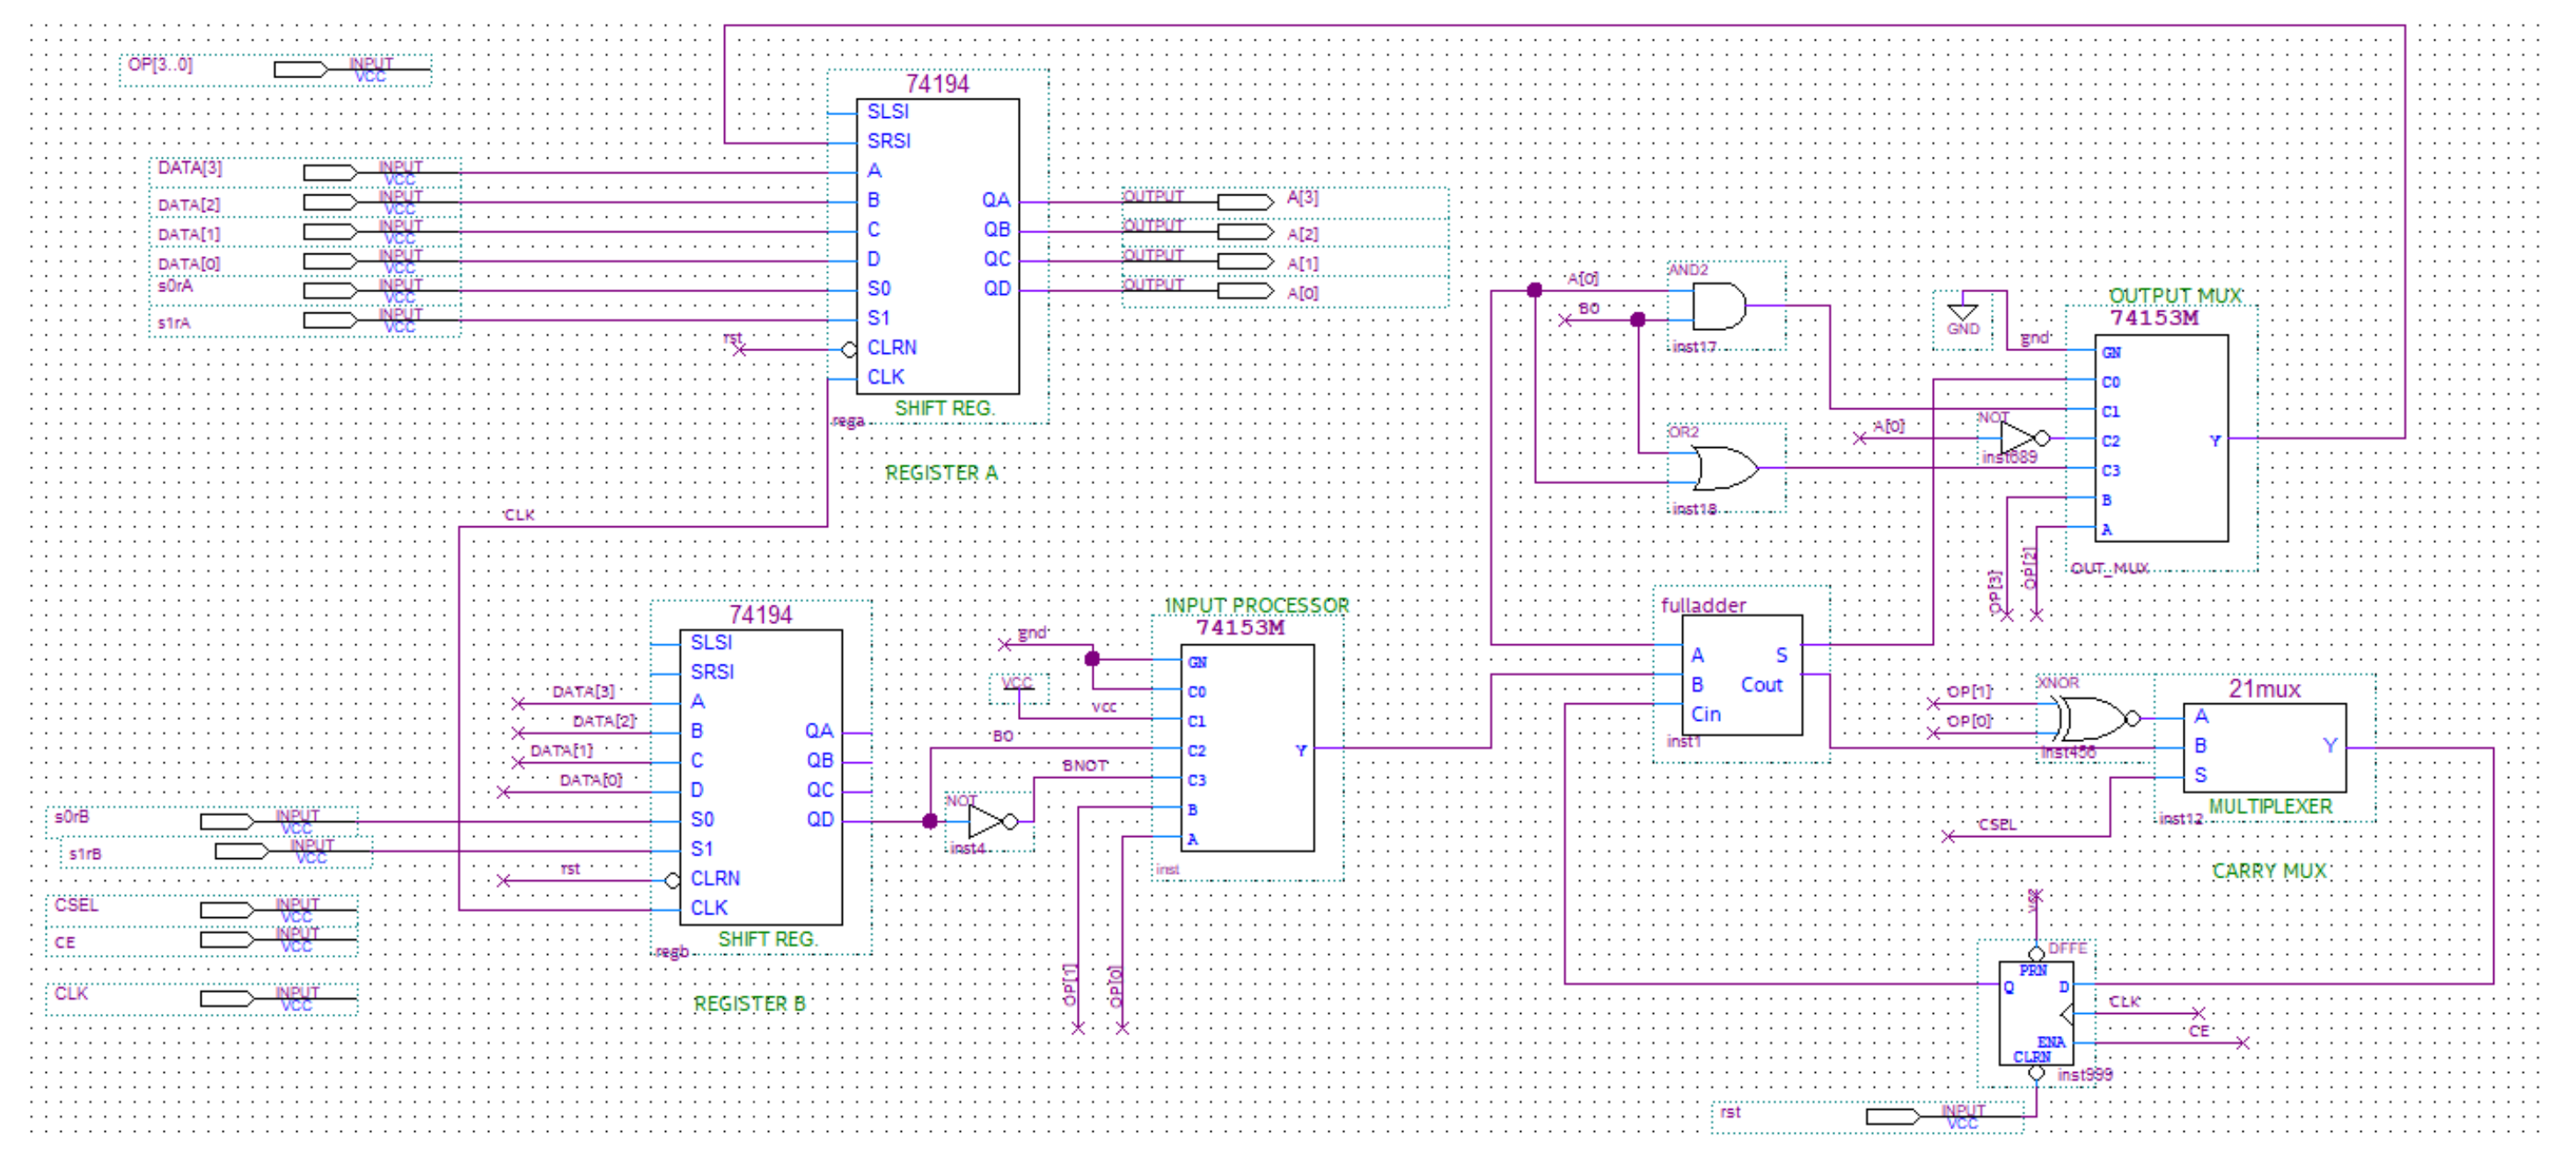
\includegraphics[height=70mm]{./ss/DATAPATH.png}
  \caption{
    Block diagram schematic of the DATAPATH module in Quartus Prime. The design includes inputs that are fed into registers, muxes, input processesors, etc.
  }
  \label{figure}
\end{figure}
 \paragraph*{DATAPATH Table}
 The following table was derived from the DATAPATH module.
  \begin{table}[h!]
      \centering
      \caption{
          Truth table that was derived from the DATAPATH module. The inputs are the 4-bit OpCodes that each represent a unique operation. This oepraiton corresponds to a certain instruction which is lsited on the far right column of the table. Note that the outputs for $x_i$ and $y_i$ each represent the 4-bit value for A and B; which make up the two integers whom of which are being operated on.
      }
      
      \begin{tabular}{c|c|c|c|c|c}%
          \toprule%%_________________________________________________________________________________________________________________________________________________________
          $ OpCode[3:0] $    &        $MUX_{OUT}$       &           $x_i$               &           $y_i$             &           $c_0$           &           $Instruction$                   \\
          \midrule%%_________________________________________________________________________________________________________________________________________________________                                   \\ \hdashline%%
              0 0 0 0        &            $c_0$          &           $A_i$               &           $0$              &           $1$             &    dec: $A - 1 \rightarrow A $            \\ \hdashline%%
              0 0 0 1        &            $c_0$          &           $A_i$               &           $1$              &           $0$             &    inc: $A + 1 \rightarrow A $            \\ \hdashline%%
              0 0 1 0        &            $c_0$          &           $A_i$               &           $B_i$            &           $0$             &    add: $A + B \rightarrow A $            \\ \hdashline%%
              0 0 1 1        &            $c_0$          &           $A_i$               &      $\overline{B_i}$      &           $1$             &    sub: $A - B \rightarrow A $            \\ \hdashline%%
              0 1 0 1        &            $c_1$          &           $A_i$               &           $1$              &           $0$             &    and: $A$ \& $B\rightarrow A $          \\ \hdashline%%
              1 0 1 0        &            $c_2$          &           $A_i$               &           $B_i$            &           $0$             &    comp: $\overline{A} \rightarrow A$     \\ \hdashline%%
              1 1 1 1        &            $c_3$          &           $A_i$               &      $\overline{B_i}$      &           $1$             &    or: A | B $\rightarrow$ A              \\ \hdashline%&
      \end{tabular}
      \label{table:1}
  \end{table}
%
\pagebreak
 \subsection*{Stage Generator}
  \paragraph*{Transition table}

\pagebreak
    \begin{table}[h!]
      \centering
      \caption{
          filler
          }
      
        \begin{tabular}{c|c|c|c|c|c}%
          \toprule%%_________________________________________________________________________________________________________________________________________________________
          $ PS $             &        $START$            &        s1rA    s0rA           &        s1rB    s0rB      &          $CSEL$           &           $CE$                   \\
          \midrule%%_________________________________________________________________________________________________________________________________________________________                                   \\ \hdashline%%
              $T_0$            &          $0$              &          $0$       $0$        &        $0$      $0$      &          $d$            &           $0$                    \\ \hdashline%%
              $T_0$            &          $1$              &          $1$       $1$        &        $d$      $d$      &          $d$            &           $d$                    \\ \hdashline%%
              $T_1$            &          $d$              &          $0$       $0$        &        $1$      $1$      &          $1$            &           $1$                    \\ \hdashline%%
              $T_2$            &          $d$              &          $0$       $1$        &        $0$      $1$      &          $0$            &           $1$                    \\ \hdashline%%
              $T_3$            &          $d$              &          $0$       $1$        &        $0$      $1$      &          $0$            &           $1$                    \\ \hdashline%%
              $T_4$            &          $d$              &          $0$       $1$        &        $0$      $1$      &          $0$            &           $1$                    \\ \hdashline%%
              $T_5$            &          $1$              &          $0$       $0$        &        $0$      $0$      &          $d$            &           $0$                    \\ \hdashline%&
              $T_5$            &          $0$              &          $0$       $1$        &        $0$      $1$      &          $0$            &           $1$                    \\ \hdashline%&
        \end{tabular}
      \label{table:1}
    \end{table}
    
\end{document}